\section{Introducción}
\label{cap:introduccion}

\subsection{Motivación y contexto}
La evolución de la domótica tradicional hacia la inteligencia ambiental (AmI, por sus siglas en inglés) representa un cambio de paradigma en la interacción humano-computadora \cite{ducatel2001ambient}. Históricamente, los sistemas de automatización residencial se han basado en un modelo reactivo, donde el usuario debe accionar comandos explícitos o establecer horarios rígidos para el control del entorno. Sin embargo, la computación sensible al contexto (\textit{context-aware computing}) persigue la creación de espacios capaces de caracterizar la situación del usuario y su entorno de forma transparente, ajustando las variables ambientales sin requerir intervención manual directa \cite{dey2001understanding}.

El despliegue de redes de sensores de bajo coste y el procesamiento local, conocido como \textit{edge computing}, ha facilitado el desarrollo de infraestructuras domóticas que preservan la privacidad del usuario al no depender exclusivamente de procesamientos centralizados en servicios en la nube \cite{shi2016edge}. A pesar de estos avances, la mayoría de implementaciones comerciales de nivel de entrada siguen empleando telemetría binaria básica, como los sensores infrarrojos pasivos (PIR). Estos dispositivos presentan limitaciones severas para determinar la presencia estática prolongada o la posición espacial exacta de un individuo, generando falsos negativos en escenarios de baja movilidad, como el estudio o el descanso \cite{labeodan2015survey}.

El presente proyecto surge ante la necesidad de desarrollar un ecosistema domótico capaz de superar dichas limitaciones volumétricas y lógicas. Mediante la integración de radares de ondas milimétricas (mmWave) \cite{soumya2023mmwave} y técnicas de fusión de sensores, se plantea la construcción de una infraestructura que actúe como un entorno proactivo, capaz de gestionar de manera autónoma la eficiencia energética, la monitorización de rutinas y la seguridad perimetral.

\begin{figure}[htbp]
    \centering
    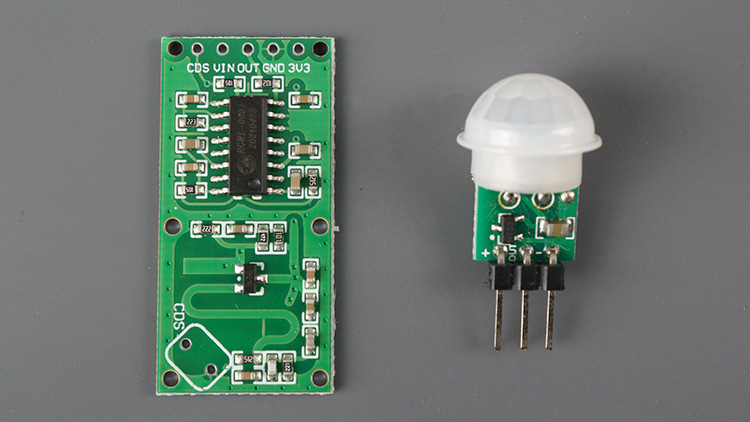
\includegraphics[width=0.6\textwidth]{Img/pir_vs_microwave.png}
    \caption{Comparativa física de componentes: módulo de radar de microondas para detección volumétrica continua (izquierda) frente a sensor infrarrojo pasivo PIR tradicional (derecha).}
    \label{fig:pir_vs_microwave_real}
\end{figure}
\section{Justificación e interés técnico}
El interés técnico de este proyecto se fundamenta en la necesidad de redefinir el paradigma actual de la automatización residencial, trasladando la carga de procesamiento desde infraestructuras dependientes de la nube hacia arquitecturas de ejecución local (\textit{edge computing}). El ecosistema predominante del internet de las cosas (IoT) a nivel de usuario depende de servidores externos para la toma de decisiones, lo que introduce latencias operativas, dependencia de la conectividad a internet y, fundamentalmente, vulnerabilidades críticas respecto a la privacidad y el control de los datos personales \cite{perera2014context}.

Este trabajo justifica la viabilidad e implementación de un sistema basado en inteligencia ambiental (AmI) operado de forma estrictamente local. Al emplear microcontroladores con firmware declarativo y un orquestador centralizado de código abierto en la propia red (como Home Assistant), se garantiza que el procesamiento algorítmico y el almacenamiento de datos no abandonen el entorno físico donde son generados, mitigando los riesgos inherentes al \textit{cloud computing} \cite{shi2016edge}.

En un segundo término, la innovación del proyecto reside en la aplicación práctica de la computación sensible al contexto (\textit{context-aware computing}). La transición de una domótica reactiva a una proactiva exige sistemas capaces de inferir el estado y las necesidades del usuario. Para ello, se aborda la complejidad del modelado del contexto mediante técnicas de fusión de sensores heterogéneos, cruzando variables lumínicas, acústicas y termohigrométricas con telemetría espacial avanzada. Es en este punto donde la integración de radares de ondas milimétricas (FMCW) resulta indispensable. Al sustituir la detección infrarroja tradicional (PIR) por tecnología capaz de registrar micromovimientos respiratorios, se eliminan los falsos negativos prolongados. Esto permite al motor algorítmico asignar estados lógicos de alta fiabilidad (como el estudio o el descanso profundo) sin requerir la interacción directa del individuo \cite{turppa2020vital}.


\subsection{Alcance y limitaciones}

\subsubsection{Alcance del proyecto}
El perímetro operativo de este Trabajo Fin de Grado comprende las siguientes actividades y entregables:
\begin{itemize}
    \item El diseño, ensamblaje y puesta en marcha de dos nodos de hardware distribuidos basados en la plataforma ESP32, equipados con sensórica biométrica y ambiental (FMCW, LDR, transductores climáticos, acústicos, etc.).
    \item La configuración e integración de la red de comunicaciones locales para el transporte de telemetría y comandos de actuación bajo entornos de red local.
    \item El desarrollo de un motor de contexto centralizado capaz de unificar las lecturas heterogéneas mediante lógica de fusión de datos, abstrayendo el comportamiento de la estancia en cuatro estados discretos.
    \item La programación y validación empírica de tres algoritmos de automatización proactiva orientados a la ergonomía visual, la higiene del sueño y la seguridad perimetral contra intrusiones.
\end{itemize}

\subsubsection{Limitaciones del sistema}
El sistema desarrollado presenta restricciones operativas que delimitan su aplicación industrial directa, las cuales se enumeran a continuación:
\begin{itemize}
    \item \textbf{Restricciones volumétricas del radar:} el sensor HLK-LD2410 posee un rango de apertura angular acotado y una distancia máxima de operación de 8 metros, lo que restringe la detección a espacios cerrados de dimensiones medias, requiriendo un estudio de ubicación crítico para evitar zonas ciegas.
    \item \textbf{Vulnerabilidad a interferencias mecánicas:} al operar mediante ondas milimétricas, el radar es susceptible a falsos positivos provocados por elementos en movimiento constante no humano, tales como ventiladores o cortinas desplazadas por corrientes de aire, requiriendo una calibración fina de umbrales por software.
    \item \textbf{Dependencia de la infraestructura de red local:} al prescindir de servicios en la nube para garantizar la privacidad, la operatividad de los nodos y el intercambio de eventos están estrictamente vinculados a la disponibilidad y estabilidad de la red de área local (WLAN) del entorno de pruebas.
    \item \textbf{Vulnerabilidades lógicas delegadas en el perímetro de red:} aunque el procesamiento local elimina los vectores de ataque externos orientados a la interceptación de datos en tránsito hacia la nube, la seguridad global del ecosistema se desplaza y delega por completo en la robustez de los mecanismos de cifrado en la red local. Aunque los microcontroladores empotrados ESP32 presentan restricciones de recursos para gestionar capas de cifrado pesado como TLS/SSL tradicional, la adopción del protocolo Noise (integrado de forma nativa en la API de ESPHome) mitiga este riesgo al cifrar la telemetría en tránsito de extremo a extremo. No obstante, un compromiso de la seguridad de la red inalámbrica doméstica (WLAN) expondría la infraestructura a potenciales ataques de denegación de servicio o suplantación de identidad física.
\end{itemize}

\subsection{Objetivos}

\subsubsection{Objetivo principal}
El objetivo fundamental de este Trabajo Fin de Grado es diseñar, implementar y validar un sistema domótico basado en inteligencia ambiental, capaz de inferir de manera continua el contexto físico y conductual del usuario para automatizar la toma de decisiones relativas al bienestar, la productividad y la seguridad en un entorno residencial, empleando hardware de bajo coste y plataformas de orquestación de código abierto.

\subsubsection{Objetivos específicos}
Para alcanzar la meta principal, se establecen los siguientes objetivos parciales:
\begin{itemize}
    \item \textbf{Diseño de hardware distribuido:} configurar y ensamblar una red de nodos de sensores y actuadores utilizando microcontroladores ESP32, garantizando la cobertura espacial del entorno de pruebas.
    \item \textbf{Implementación de telemetría avanzada:} sustituir la detección de presencia tradicional por telemetría espacial continua, empleando radares de ondas milimétricas (HLK-LD2410) combinados con mediciones lumínicas (LDR) y ambientales.
    \item \textbf{Desarrollo del motor de contexto:} programar un orquestador centralizado que, mediante técnicas de fusión de datos, asigne un estado unívoco a la habitación (ocio, estudio, durmiendo, ausente) en tiempo real.
    \item \textbf{Automatización proactiva y seguridad:} diseñar algoritmos de control lógico para la gestión ergonómica de la iluminación, la evaluación del descanso y el despliegue de un sistema de alarma robusto frente a vulnerabilidades lógicas, como las condiciones de carrera.
    \item \textbf{Validación e integración:} evaluar el comportamiento de la arquitectura propuesta en escenarios de uso real, aplicando redundancias lógicas para verificar la tolerancia a fallos del hardware.
\end{itemize}

\subsection{Metodología empleada}
Para la consecución de los objetivos propuestos, se ha adoptado una metodología de ingeniería basada en el ciclo de vida en V para sistemas empotrados y de IoT, adaptada a desarrollos iterativos \cite{sommerville2011software}. Este enfoque metodológico estructura el proyecto en fases de abstracción descendente seguidas de fases de verificación ascendente, asegurando que cada componente implementado responda directamente a un requisito previamente especificado, como se ilustra gráficamente en la Figura \ref{fig:ciclo_v}.

La metodología se despliega a través de las siguientes fases secuenciales:
\begin{enumerate}
    \item \textbf{Ingeniería de requisitos y restricciones:} definición formal de las necesidades funcionales y de las fronteras físicas del entorno para acotar la selección de componentes.
    \item \textbf{Diseño de la arquitectura e integración de hardware:} fase donde se proyecta la topología de red y se realiza el ensamblaje electrónico, aplicando técnicas de instrumentación en frío y en caliente (uso de multímetros para validación de la caída de potencial en los divisores de tensión de los sensores) para garantizar la estabilidad eléctrica.
    \item \textbf{Desarrollo del firmware y lógica de abstracción:} programación de los microcontroladores mediante abstracciones de hardware declarativas, optimizando los intervalos de actualización y los rangos de atenuación analógica.
    \item \textbf{Orquestación y fusión de datos en el Edge:} implementación de las máquinas de estado y reglas lógicas redundantes en el nodo central para dotar al sistema de tolerancia a fallos ante pérdidas temporales de conectividad o lecturas anómalas de los transductores.
    \item \textbf{Fase de pruebas experimentales y evaluación técnica:} protocolo de validación que abarca desde pruebas unitarias en caja negra hasta pruebas de integración en escenarios reales de uso continuo, analizando la fiabilidad de las transiciones de estado.
\end{enumerate}

    \begin{figure}[htbp]
    \centering
    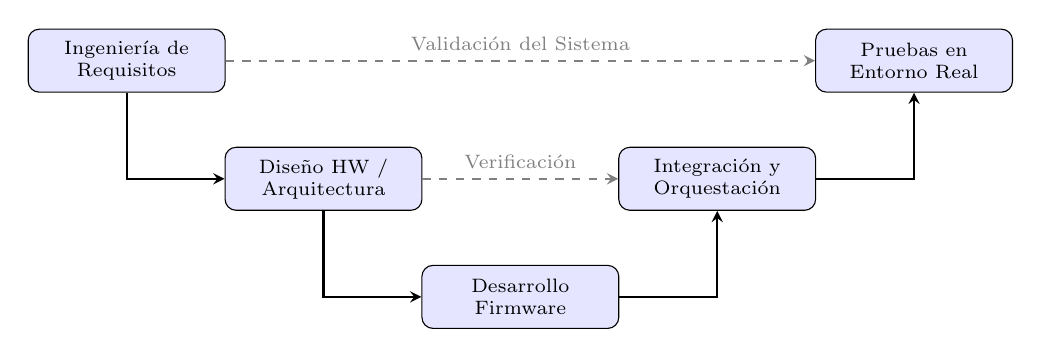
\begin{tikzpicture}[
        box/.style={draw, rectangle, rounded corners, minimum width=2.5cm, minimum height=0.8cm, align=center, fill=blue!10, font=\scriptsize},
        arrow/.style={thick, -stealth}
    ]
    
    % Explicit coordinates to guarantee it fits the page
    \node[box] (req) at (0, 4) {Ingeniería de\\Requisitos};
    \node[box] (arch) at (2.5, 2.5) {Diseño HW /\\Arquitectura};
    \node[box] (firm) at (5, 1) {Desarrollo\\Firmware};
    
    \node[box] (integ) at (7.5, 2.5) {Integración y\\Orquestación};
    \node[box] (test) at (10, 4) {Pruebas en\\Entorno Real};
    
    % Connections down
    \draw[arrow] (req) |- (arch);
    \draw[arrow] (arch) |- (firm);
    
    % Connections up
    \draw[arrow] (firm) -| (integ);
    \draw[arrow] (integ) -| (test);
    
    % Horizontal verification arrows (dashed)
    \draw[thick, dashed, color=gray, -stealth] (arch) -- node[anchor=south, font=\scriptsize] {Verificación} (integ);
    \draw[thick, dashed, color=gray, -stealth] (req) -- node[anchor=south, font=\scriptsize] {Validación del Sistema} (test);
    
    \end{tikzpicture}
    \caption{Adaptación del modelo del ciclo de vida en V para la metodología de desarrollo de este Trabajo Fin de Grado.}
    \label{fig:ciclo_v}
\end{figure}

\subsection{Estructura de la memoria}
El presente documento se estructura en distintos capítulos organizados para detallar la progresión del proyecto:

El Capítulo 1 introduce el contexto tecnológico, la problemática existente y los objetivos propuestos. El Capítulo 2 presenta la evolución de la domótica y el estado del arte de las tecnologías implicadas. El Capítulo 3 define el problema a resolver y analiza los requisitos del sistema, tanto funcionales como no funcionales. El Capítulo 4 detalla el diseño del sistema, abarcando su arquitectura y modelado lógico. El Capítulo 5 expone la selección e integración de las tecnologías de hardware y software empleadas. El Capítulo 6 describe el plan de implantación y las pruebas realizadas durante el despliegue. El Capítulo 7 realiza una evaluación del sistema desde el punto de vista técnico, económico y de sostenibilidad. El Capítulo 8 recoge el presupuesto del proyecto. El Capítulo 9 presenta los planos y esquemas de la infraestructura. Finalmente, el Capítulo 10 recoge las conclusiones derivadas del trabajo y expone las futuras líneas de investigación. Adicionalmente, se incluyen una serie de anexos con los manuales de usuario y técnicos correspondientes.